\subsection{Teledetección}

La teledetección, en inglés ``Remote Sensing'', se aplica en una diversidad de campos disciplinarios. Esta tecnología transversal se utiliza en ámbitos como la geología, la meteorología, la ecología, la oceanografía, la agricultura y la planificación urbana, por nombrar algunos \cite{schowengerdt2006remote}.

Dada su aplicación transversal en múltiples disciplinas, la teledetección ha sido objeto de diversas definiciones propuestas por distintos autores. Un ejemplo destacado es el de \citeA{canada2007fundamentals}, quien define a la teledetección como "La ciencia (y hasta cierto punto, arte) de adquirir información sobre la superficie de la Tierra sin estar en contacto directo con ella. Esto se realiza detectando y registrando la energía reflejada o emitida, y procesando, analizando y aplicando dicha información".

Otros autores, como \citeA{chuvieco2016fundamentals}, definen la teledetección como una disciplina centrada en la captura de información sobre objetos terrestres utilizando sensores remotos. Estos instrumentos se encargan de recoger la energía electromagnética, que puede presentarse como radiación reflejada o emitida por la superficie terrestre.

En pocas palabras, la teledetección puede describirse como un campo de estudio basado en la adquisición y procesamiento de información de la superficie terrestre sin la necesidad de estar presente en el lugar estudiado. Su enfoque reside en la interpretación de la radiación electromagnética, un proceso que facilita la observación y recopilación de datos sobre las propiedades y características de la superficie terrestre.

La teledetección tiene como objetivo principal la generación de información relevante para la toma de decisiones o gestión de recursos sobre un determinado fenómeno o área de interés, a partir del procesamiento de la información captada por sensores remotos.

\begin{figure}[H]
    \begin{center}
        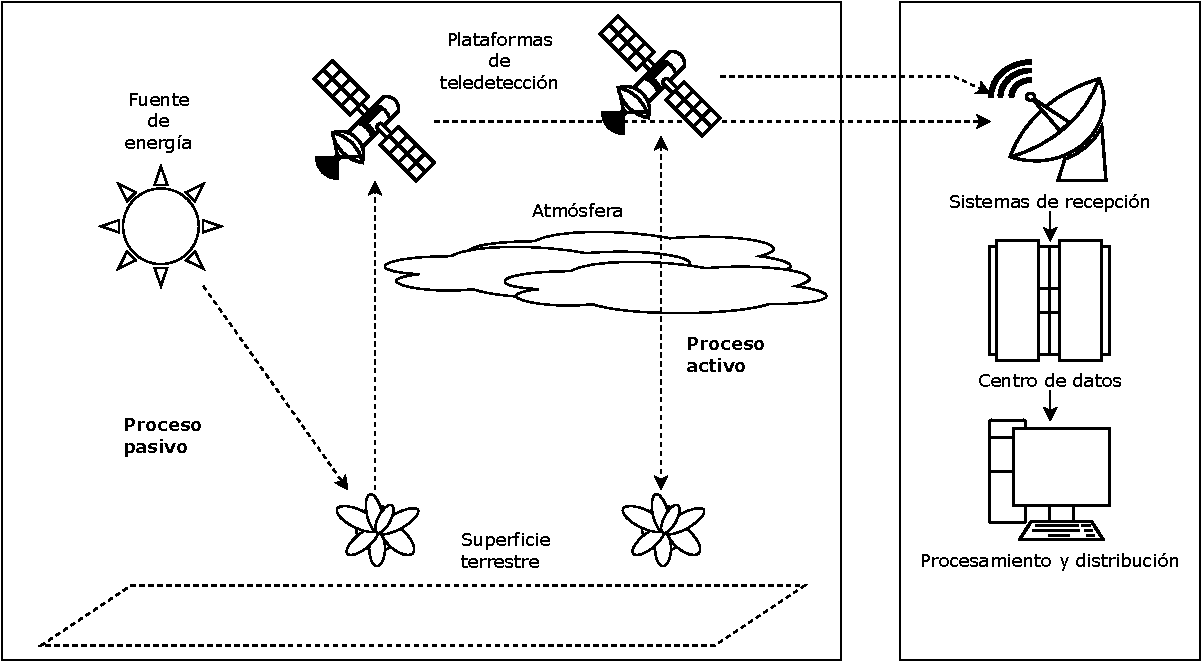
\includegraphics[width=1\textwidth]{Images/Teledeteccion.pdf}
    \end{center}
    \caption{Flujo de la información en un proceso de teledetección.}
    \reference{Elaborado por el autor.}
    \label{fig:Teledeteccion}
\end{figure}

El proceso de teledetección, como se muestra en la Figura~\ref{fig:Teledeteccion}, es un enfoque multidisciplinario que involucra múltiples factores fundamentales para llevar a cabo diversas tareas específicas. Según \citeA{chuvieco2016fundamentals}, este proceso se compone de seis componentes principales:

\begin{enumerate}
    \item \textbf{Fuente de energía}: Este componente se refiere a la fuente que genera la radiación electromagnética que interactúa entre el sensor y la superficie. Principalmente, la fuente más relevante es el Sol, ya que proporciona iluminación y calor a nuestro planeta.
    \item \textbf{Superficie terrestre}: Incluye vegetación, suelos, agua, rocas, nieve, hielo y estructuras humanas. Estas superficies reciben la energía procedente de la fuente y, debido a la interacción física y química con la energía entrante, reflejan y emiten una parte de esa energía de vuelta al sensor satelital. La atmósfera puede filtrar parte o toda la energía, dependiendo de sus concentraciones de gas y partículas.
    \item \textbf{Sensor y plataforma}: El sensor es el dispositivo que mide y registra la energía proveniente de la superficie. La plataforma proporciona los servicios esenciales para el funcionamiento del sensor, como el control de actitud y órbita, suministro de energía y comunicación con el sistema de recepción terrestre. Los satélites son los más comunes en este sentido. Usualmente, un satélite de observación de la Tierra incluye distintos sensores, dependiendo de su misión principal. Los satélites meteorológicos, por ejemplo, suelen tener sensores para detectar humedad atmosférica, temperatura, albedo, ozono o concentraciones de aerosoles.
    \item \textbf{Sistema de recepción en tierra}: Este componente recoge los datos digitales brutos medidos por el sensor, los almacena y los formatea de manera adecuada. El sistema terrestre realiza algunas correcciones de preprocesamiento básicas antes de distribuir las imágenes.
    \item \textbf{Analista}: Es la persona encargada de transformar los datos de la imagen procesada en información temática de interés, utilizando técnicas visuales y/o digitales (en éste último caso, haciendo uso de tecnología especializada, como servidores, dispositivos geodésicos, o estaciones de trabajo).
    \item \textbf{Comunidad de usuarios}: Es el grupo que utiliza la información extraída de los datos originales para una amplia gama de aplicaciones.
\end{enumerate}

\subsubsection{Radiación electromagnética}

Tal como se mencionó anteriormente, para realizar teledetección, es esencial contar con una fuente de energía que ilumine el blanco de estudio, a menos que el propio blanco sea el que emita la energía que se pretende medir. Dicha energía se presenta en forma de radiación electromagnética \cite{canada2007fundamentals}.

Toda materia que posee una temperatura absoluta superior a cero emite energía electromagnética debido a la agitación molecular. La temperatura absoluta se mide convencionalmente en Kelvin ($K$), con incrementos escalados en grados Celsius ($^{\circ}$C). El cero absoluto, que se representa como $0K = -273.15 ^{\circ}C$, es la temperatura más baja alcanzable, en la cual las moléculas cesan completamente su movimiento. Cuando la temperatura de un objeto o sustancia aumenta, las moléculas que lo componen se vuelven más activas y se agitan con mayor intensidad. Esta agitación molecular produce una emisión de energía en forma de radiación electromagnética, la cual puede manifestarse en diversas formas, como luz visible, radiación infrarroja o incluso radiación de alta frecuencia, como los rayos X y los rayos gamma \cite{tempfli2009principles}.

La radiación electromagnética es una forma de energía que se propaga a través de ondas o partículas llamadas fotones. Las propiedades de la radiación electromagnética pueden ser explicadas por dos teorías: La teoría de ondas de la luz y la teoría cuántica \cite{chuvieco2016fundamentals}.

Según la teoría de ondas de la luz, la radiación electromagnética se compone de un campo eléctrico (E) que cambia en su intensidad en una dirección perpendicular al camino que sigue la radiación, y un campo magnético (M) que se ubica en un ángulo de 90 grados respecto al campo eléctrico \cite{canada2007fundamentals}. Ambos campos se desplazan a una velocidad de aproximadamente $c = 3 \times 10^8 \, \mathrm{m/s^{-1}}$ que corresponde a la velocidad de la luz \cite{chuvieco2016fundamentals}.

\begin{figure}[H]
    \begin{center}
        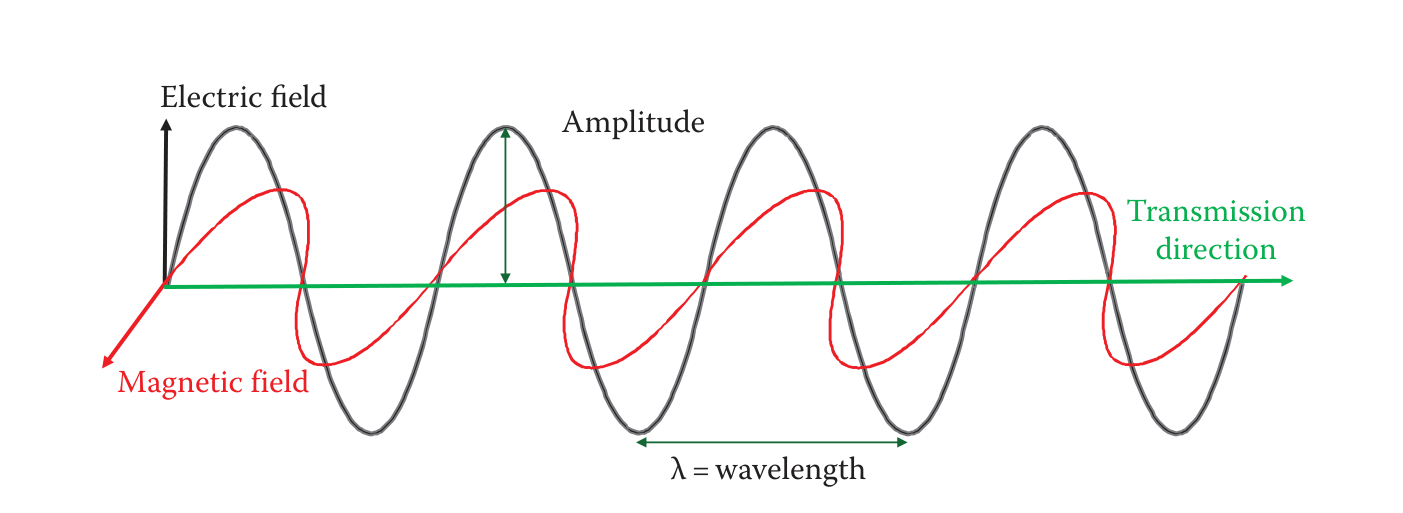
\includegraphics[width=1\textwidth]{Images/ComponentesRadiacionElectromagnetica.png}
    \end{center}
    \caption{Propagación de la radiación electromagnética y sus componentes eléctricos y magnéticos oscilantes.}
    \reference{Datos tomados de \citeA{chuvieco2016fundamentals}.}
    \label{fig:ComponentesRadiacionElectromagnetica}
\end{figure}

Como se muestra en la Figura~\ref{fig:ComponentesRadiacionElectromagnetica}, la radiación electromagnética oscila en un dirección específica. Estas ondas pueden ser descritas en función de su longitud (\(\lambda\)) y su frecuencia (\(\nu\)), las cuales están relacionadas por:

\begin{equation}
    \label{eq:LongitudOndaFrecuencia}
    c = \lambda \times \nu
\end{equation}

donde:
\begin{itemize}
    \item $c$ es la velocidad de la luz $(3 \times 10^8 \, \mathrm{m/s^{-1}})$.
    \item \(\lambda\) es la longitud de onda o la distancia entre dos picos sucesivos (generalmente en micrómetros, 1 $\mu$m = \(10^{-6}\) m; o nanómetros, 1 $n$m = \(10^{-9}\) m).
    \item \(\nu\) es la frecuencia, o el número de ciclos que pasan por un punto fijo por unidad de tiempo (en hercios, ciclos $s^{-1}$).
\end{itemize}

Por otro lado, según la teoría cuántica de la luz, la radiación se describe como una secuencia de paquetes de energía discretos conocidos como fotones o cuantos, los cuales tienen una masa igual a cero. La cantidad de energía transportada por un fotón es directamente proporcional a su frecuencia:

\begin{equation}
    \label{eq:TeoriaCuanticaLuz}
    E = h \times \nu
\end{equation}

donde:
\begin{itemize}
    \item $E$ es la energía radiante de un fotón (en joules, $J$).
    \item \(\nu\) es la frecuencia.
    \item $h$ es la constante de Planck (\(6.626 \times 10^{-34} \, \mathrm{J \, s}\)).
\end{itemize}

La ecuación de la energía de un fotón en términos de la velocidad de la luz y la longitud de onda de la onda electromagnética se expresa como:

\begin{equation}
    E = \frac{{h \times c}} {{\lambda}}
\end{equation}

donde:

\begin{itemize}
    \item $E$ es la energía radiante de un fotón (en joules, $J$).
    \item $c$ es la velocidad de la luz $(3 \times 10^8 \, \mathrm{m/s^{-1}})$.
    \item $h$ es la constante de Planck (\(6.626 \times 10^{-34} \, \mathrm{J \, s}\)).
    \item \(\lambda\) es la longitud de onda o la distancia entre dos picos sucesivos (generalmente en micrómetros, 1 $\mu$m = \(10^{-6}\) m; o nanómetros, 1 $n$m = \(10^{-9}\) m).
\end{itemize}

Por lo tanto, existe una relación inversa entre la longitud de onda y la frecuencia de una radiación. A medida que la longitud de onda aumenta o la frecuencia disminuye, el contenido de energía también disminuye (ver Figura~\ref{fig:RelacionLongitudOnda}). Esto implica que la detección de radiaciones de longitud de onda larga se vuelve más difícil en comparación con las de longitud de onda corta, ya que las primeras tienen menos energía y requieren métodos de detección más sensibles \cite{chuvieco2016fundamentals}

\begin{figure}[H]
    \begin{center}
        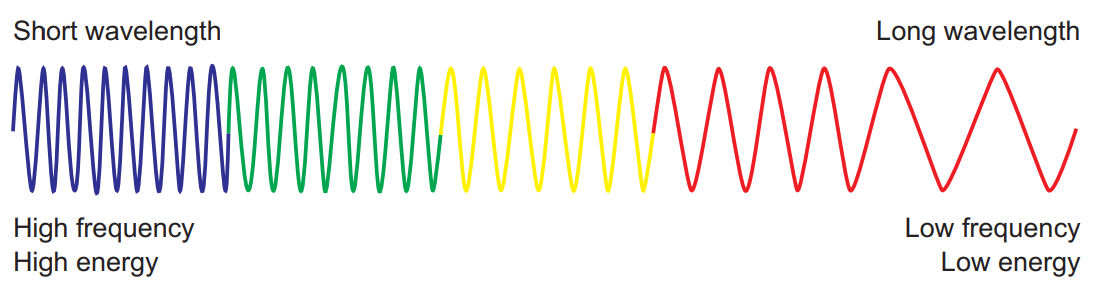
\includegraphics[width=1\textwidth]{Images/RelacionLongitudOnda.png}
    \end{center}
    \caption{Relación inversa entre la longitud de onda y la frecuencia.}
    \reference{Datos tomados de \citeA{tempfli2009principles}.}
    \label{fig:RelacionLongitudOnda}
\end{figure}

Las radiaciones de mayor energía y menor longitud de onda son los rayos gamma y los rayos X, utilizados en aplicaciones médicas y observación astronómica, mientras que las radiaciones de menor energía y mayor longitud de onda se utilizan en las telecomunicaciones, radio y televisión \cite{chuvieco2016fundamentals}. Estas diferentes formas de radiación se distribuyen a través de un amplio rango de frecuencias y longitudes de onda, conocido como espectro electromagnético.

\subsubsection{Espectro electromagnético}

El espectro electromagnético es la distribución de energías de las radiaciones electromagnéticas, se extiende desde los rayos gamma, que son de longitud de onda extremadamente corta $10^-11 m$, hasta las ondas de radio de gran longitud $10^5m$ \cite{joseph2005fundamentals}.

\begin{figure}[H]
    \begin{center}
        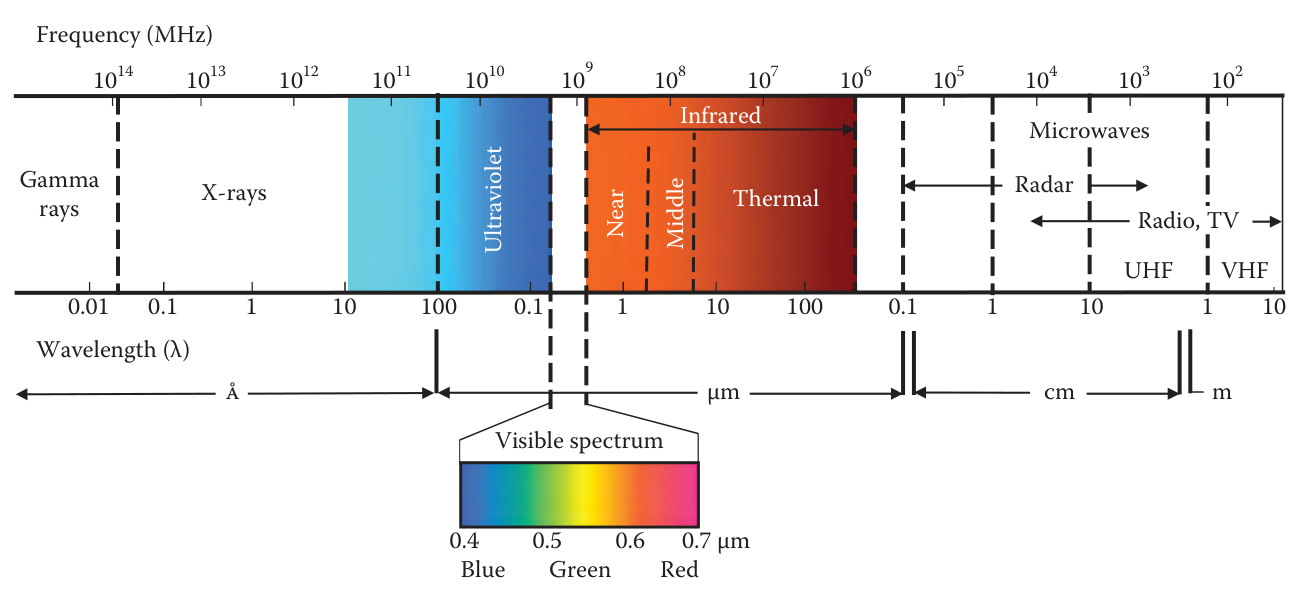
\includegraphics[width=1\textwidth]{Images/EspectroElectromagnetico.png}
    \end{center}
    \caption{Espectro electromagnético.}
    \reference{Datos tomados de \citeA{chuvieco2016fundamentals}.}
    \label{fig:EspectroElectromagnetico}
\end{figure}

La Figura~\ref{fig:EspectroElectromagnetico} muestra el espectro electromagnético, que está dividido en diversas regiones, cada una denotando un comportamiento distinto de las ondas electromagnéticas durante los procesos de emisión, transmisión y absorción.

En el espectro electromagnético, la región de los rayos gamma es caracterizada por ondas con frecuencias que suelen ser mayores a $10^{19}$ Hz, y longitudes de onda menores a $10^{-11}$  \cite{chuvieco2016fundamentals}. Dicha región alberga una gran cantidad de energía, lo suficiente para alterar la estructura de los átomos y moléculas. Esta capacidad puede generar mutaciones genéticas y condiciones carcinógenas en organismos vivos. Los rayos gamma, debido a su elevada energía y capacidad de penetración, son una considerable amenaza para la salud y la seguridad.

Posteriormente en el espectro, los rayos X se sitúan con frecuencias generalmente en el rango de $10^{16}$ Hz a $10^{19}$ Hz, y longitudes de onda entre $10^{-8}$ m y $10^{-11}$ m. Los rayos X son ampliamente utilizados en la medicina debido a su capacidad para atravesar los tejidos del cuerpo humano, lo que permite obtener imágenes de alta resolución de las estructuras internas para diagnósticos y tratamientos médicos.

En el extremo opuesto del espectro electromagnético se ubican las ondas con frecuencias más bajas, y longitudes de onda más largas. Esta sección del espectro es vital para las telecomunicaciones, ya que estas ondas pueden recorrer grandes distancias con mínima pérdida de energía y tienen la capacidad de difractarse alrededor de obstáculos. Estas características hacen que estas ondas sean ideales para la transmisión de información a larga distancia, encontrando uso en servicios como la radiodifusión, la televisión y la telefonía móvil.

En cuanto a las regiones del espectro electromagnético que son utilizadas para tareas de teledetección, generalmente se emplean las áreas desde el ultravioleta hasta las microondas \cite{chuvieco2016fundamentals}. Cada una de estas regiones, y las intermedias, ofrece a la teledetección una serie de capacidades únicas debido a las diferentes características de las ondas electromagnéticas que se encuentran en cada una. Las diferencias en frecuencia, longitud de onda y energía entre las distintas regiones del espectro, resultan en variaciones en la forma en que estas ondas interactúan con la atmósfera y con la superficie terrestre, proporcionando una diversidad de información en la teledetección.

Las regiones del espectro electromagnético que se emplean en teledetección son:

\begin{itemize}

    \item \textit{Región Ultravioleta (UV)}: Justo antes del espectro visible, presenta longitudes de onda más breves que la luz visible y más largas que los rayos X. Esta se ubica después del segmento violeta del espectro visible, de ahí su denominación. La radiación UV, mayormente absorbida por la atmósfera terrestre, cuando es detectada, puede brindar datos significativos para investigar la atmósfera, la capa de ozono y los efectos biológicos de la radiación solar. Ciertos materiales en la superficie terrestre, principalmente piedras y minerales, emiten luz visible al estar expuestos a radiación UV, fenómeno denominado fluorescencia, lo que facilita su identificación y estudio \cite{canada2007fundamentals}.

    \item \textit{Región del Espectro Visible (VIS)}: Engloba las longitudes de onda que el ojo humano puede captar y donde la energía solar es más intensa \cite{chuvieco2016fundamentals}. El espectro visible se puede descomponer en tres colores fundamentales: azul (0.4-0.5 µm), verde (0.5-0.6 µm) y rojo (0.6-0.7 µm) \cite{canada2007fundamentals}. Esta región visible es particularmente útil para examinar fenómenos como la vegetación, la transparencia del agua y la composición del suelo.

    \item \textit{Región del Infrarrojo Cercano (NIR)}: Esta región se localiza justo fuera del límite de percepción humana y se la conoce como infrarrojo reflectante o fotográfico. Una sección de esta región espectral (0.7-0.9 $\mu m$) puede ser detectada usando películas especiales. El NIR es relevante por su sensibilidad para determinar el estado de salud de las plantas y la humedad del suelo \cite{tempfli2009principles,emery2017introduction}.

    \item \textit{Región del Infrarrojo Medio (MIR)}: Esta región espectral se ubica entre las regiones NIR y TIR.

          \begin{enumerate}
              \item De 1.2 a 2.5 µm, la influencia de la energía solar es aún muy notable, comúnmente conocida como la región SWIR \cite{tempfli2009principles}. Esta región proporciona las mejores estimaciones de la humedad, contenido de suelo y vegetación \cite{chuvieco2016fundamentals}.
              \item De 3 a 8 µm, la señal se vuelve una mezcla de energía solar reflejada y energía emitida por la superficie, siendo el componente emitido más destacado conforme las longitudes de onda se expanden. \item El intervalo de 3-5 µm es especialmente útil para detectar fuentes de alta temperatura, como volcanes o incendios \cite{chuvieco2016fundamentals}.
          \end{enumerate}

    \item \textit{La región del Infrarrojo Térmico (TIR)}: Abarca la energía emitida por la superficie terrestre y se emplea para mapear las temperaturas superficiales, detectar la evapotranspiración de la vegetación, analizar propiedades de hielos y nubes, estudiar el impacto del calor urbano y distinguir tipos de rocas \cite{canada2007fundamentals,emery2017introduction}.

    \item \textit{Región de las Microondas (MW)}: En esta región espectral operan los sistemas de radar de imágenes. Su ventaja principal es la baja absorción atmosférica, características por el cual, se puede obtener información a través de las nubes. La radiación de microondas también puede penetrar las copas de los bosques hasta varias profundidades y son muy útiles para discriminar vegetación, cobertura de nieve, rugosidad superficial, dirección de las olas o la forma y orientación de los hidrómetros atmosféricos \cite{emery2017introduction}.

\end{itemize}

Cada una de estas regiones del espectro electromagnético presenta características y ventajas únicas para la teledetección, permitiendo la recopilación de datos que pueden ser empleados en una variedad de aplicaciones.

\subsubsection{Interacción de la radiación electromagnética con la atmósfera}

El sol, siendo una de las fuentes primordiales de energía electromagnética, juega un papel crucial en el sustento de la vida en la Tierra. No obstante, para que su radiación llegue a la superficie terrestre, es necesario que atraviese una considerable extensión de la atmósfera \cite{tempfli2009principles}.

La constitución de la atmósfera es sumamente diversa, incluyendo gases tales como nitrógeno ($N$, representando el 78\% de la atmósfera), oxígeno ($O_{2}$, con un 21\%), argón ($Ar$, alrededor del 0.9\%), vapor de agua ($H_{2}O$, aproximadamente 0.04\%), dióxido de carbono ($CO_{2}$, alrededor del 0.033\%) y ozono ($O_{3}$, un 0.012\%). No solo se componen de gases, también existen partículas sólidas en suspensión, denominadas aerosoles, que interactúan activamente con la radiación electromagnética. Estos aerosoles abarcan una variedad de sustancias, desde sal oceánica hasta partículas de polvo, carbono y residuos de combustión \cite{chuvieco2016fundamentals}.

\begin{figure}[H]
    \begin{center}
        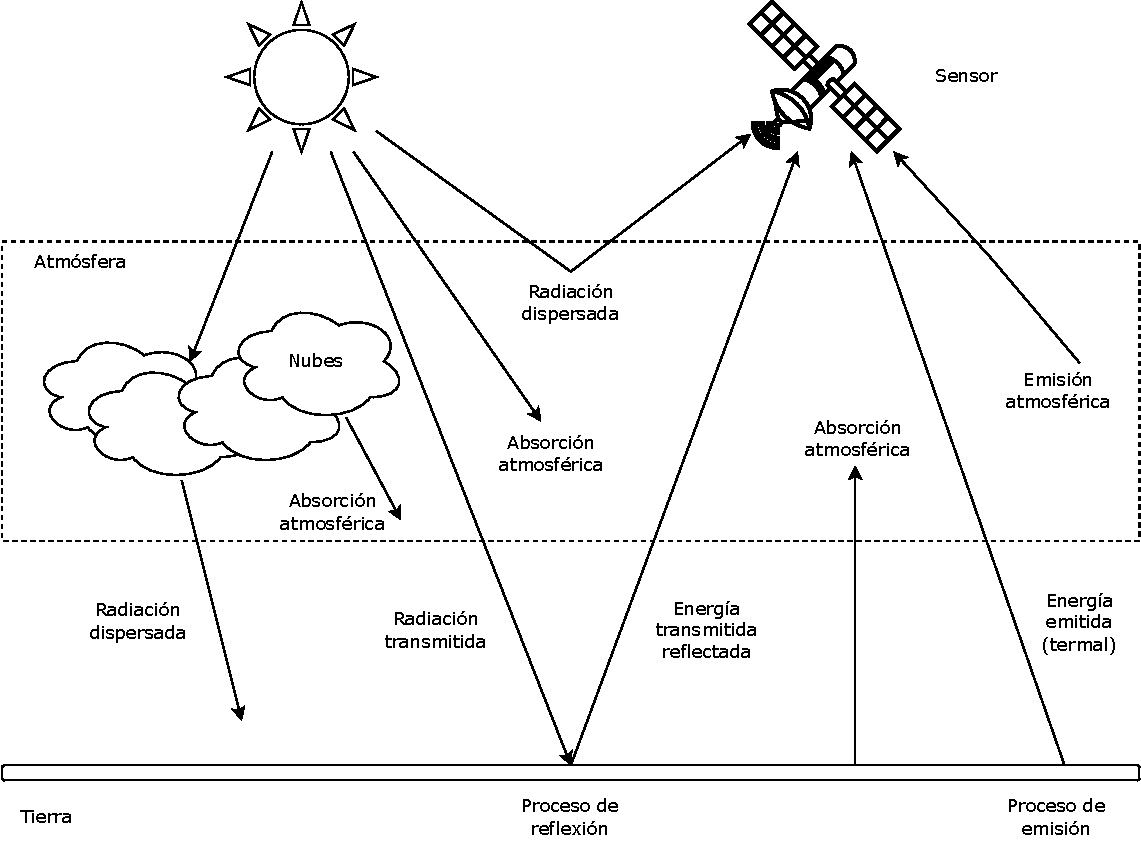
\includegraphics[width=1\textwidth]{Images/InteraccionAtmosfera.pdf}
    \end{center}
    \caption{Ventanas atmosféricas vistas a través del porcentaje de transmisión atmosférica.}
    \reference{Datos tomados de \citeA{tempfli2009principles}.}
    \label{fig:InteraccionAtmosfera}
\end{figure}

Los efectos de estos elementos atmosféricos pueden clasificarse en tres categorías distintas: Absorción, Dispersión, y Emisión \cite{chuvieco2016fundamentals}, tal y como se puede ver en la Figura~\ref{fig:InteraccionAtmosfera}.

\textbf{a) Absorción y transmisión atmosférica}

El fenómeno de absorción actúa como un filtro selectivo, ya que las moléculas presentes en la atmósfera absorben energía en diferentes longitudes de onda. Algunas de las causas de esta filtración son los componentes atmosféricos como el oxígeno atómico, el ozono, el vapor de agua y el dióxido de carbono \cite{chuvieco2016fundamentals}. En contraparte, el fenómeno de transmisión permite que ciertas longitudes de onda de la radiación electromagnética atraviesen la atmósfera sin ser absorbidas significativamente. Estas longitudes de onda no encuentran obstáculos en su camino hacia la superficie terrestre, lo que permite su detección y registro por parte de los sensores remotos \cite{canada2007fundamentals}.

Dado que los sensores remotos están diseñados para observar la superficie terrestre, su sensibilidad se enfoca en las regiones donde la absorción es baja (alta transmisión]), conocidas como ventanas atmosféricas: visible (VIS), infrarrojo cercano (NIR), infrarrojo de onda corta (SWIR), infrarrojo medio (MIR), infrarrojo térmico (TIR) y microondas (> 1 cm), tal y como se ve en la Figura~\ref{fig:VentanasAtmosféricas}. Aunque la transmisión generalmente es alta, no alcanza el 100\% debido a condiciones atmosféricas como la presencia de nubes (que dificultan la observación en las bandas solares y térmicas) y partículas sólidas que reducen la visibilidad a largas distancias debido a la absorción \cite{emery2017introduction}. La mayoría de los sensores están adaptados a estas ventanas atmosféricas debido a su función principal de observar la superficie terrestre \cite{canada2007fundamentals,chuvieco2016fundamentals}. Sin embargo, en los últimos años se han desarrollado nuevos sensores capaces de penetrar la atmósfera en cualquier condición, empleando longitudes de onda de entre 1$cm$ y 1$m$, es decir microondas \cite{emery2017introduction}.

\begin{figure}[H]
    \begin{center}
        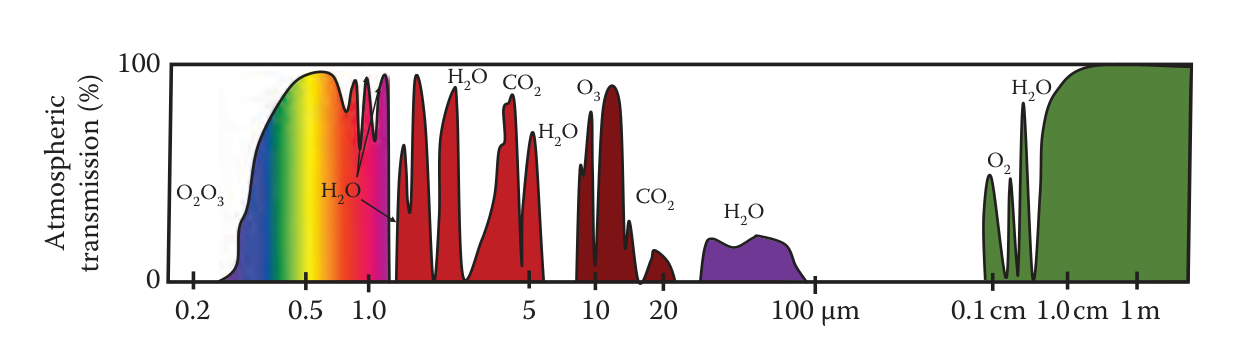
\includegraphics[width=1\textwidth]{Images/VentanasAtmosfericas.png}
    \end{center}
    \caption{Ventanas atmosféricas vistas a través del porcentaje de transmisión atmosférica.}
    \reference{Datos tomados de \citeA{chuvieco2016fundamentals}.}
    \label{fig:VentanasAtmosféricas}
\end{figure}

\textbf{b) Dispersión atmosférica}

Este fenómeno sucede cuando el entorno atmosférico, compuesto por diversos gases, aerosoles y vapor de agua, interactúa directamente con la radiación electromagnética, ocasionando que esta se desvíe de su trayectoria original \cite{canada2007fundamentals}.

La diversidad de los tamaños de las partículas presentes en la atmósfera da lugar a diferentes tipos de dispersión: Rayleigh, Mie y la dispersión no selectiva.

\textit{Dispersión de Rayleigh}: La dispersión de Rayleigh es especialmente sensible a la longitud de onda de la radiación incidente, lo cual afecta significativamente a las bandas de longitud de onda más corta. Esta dispersión se da cuando la radiación electromagnética interactúa con partículas que son más pequeñas que las longitudes de onda, como por ejemplo, las de moléculas de nitrógeno ($NO_{2}$) y oxígeno ($O_{2}$) \cite{tempfli2009principles, chuvieco2016fundamentals}. Un ejemplo claro de este tipo de dispersión es el cielo, ya que debido a la longitud de onda más corta dentro del espectro visible, se puede ver el cielo azul \cite{canada2007fundamentals}, tal y como se puede ver en la Figura~\ref{fig:DispersionRayleigh}.

\begin{figure}[H]
    \begin{center}
        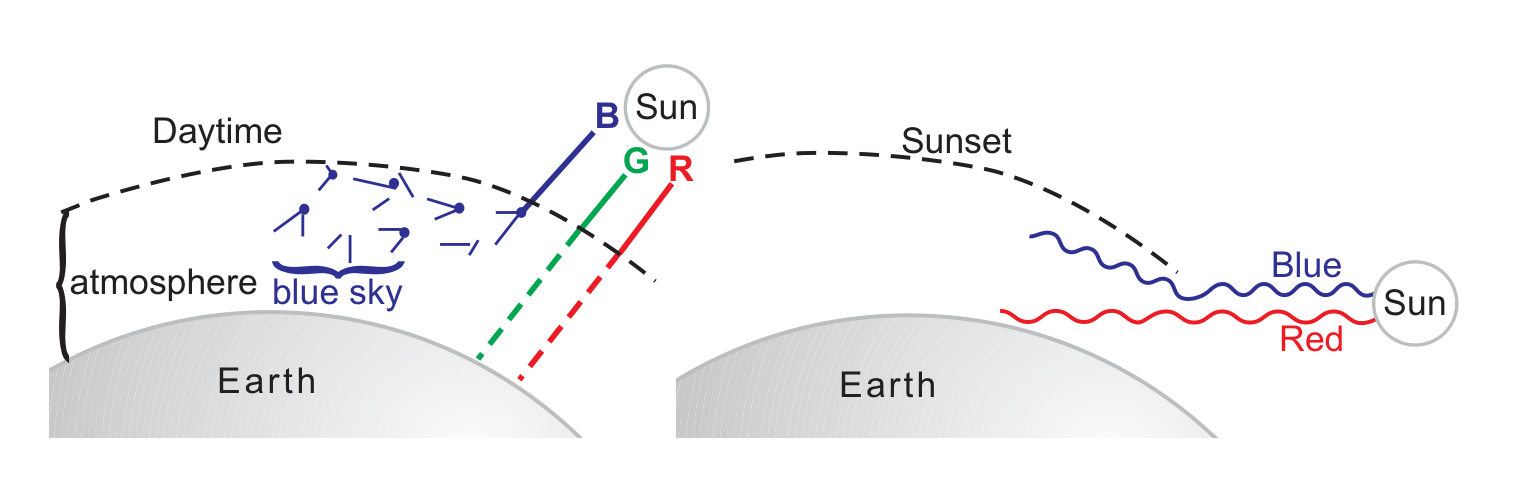
\includegraphics[width=1\textwidth]{Images/DispersionRayleigh.png}
    \end{center}
    \caption{Efectos de la dispersión de Rayleigh en el color del cielo.}
    \reference{Datos tomados de \citeA{tempfli2009principles}.}
    \label{fig:DispersionRayleigh}
\end{figure}

La dispersión de Rayleigh perturba la percepción remota en el rango espectral visible, particularmente desde altitudes elevadas. Esta interrupción provoca una distorsión en las características espectrales de la luz reflejada, resultando en una sobreestimación de las longitudes de onda más cortas y una tonalidad azulada en las imágenes capturadas, especialmente cuando se usan sensores multiespectrales \cite{tempfli2009principles}.

\textit{Dispersión de Mie}: Depende también de la longitud de onda incidente, pero su influencia es menor en comparación con la radiación de Rayleigh. Ocurre generalmente cuando las partículas tienen aproximadamente el mismo tamaño de la longitud de onda de la radiación \cite{canada2007fundamentals}. Esta dispersión se da generalmente en la atmósfera baja, donde hay una mayor abundancia de partículas grandes, y domina en condiciones de nubes cubiertas, teniendo un influencia en en el rango espectral desde el cercano ultravioleta hasta el infrarrojo medio \cite{tempfli2009principles}. En este tipo de dispersión, los elementos que son especialmente responsables son las partículas de aerosoles y el polvo atmosférico. Sin embargo, otros elementos como incendios forestales o niebla costera pueden ocasionarla \cite{chuvieco2016fundamentals}.

\textit{Dispersión no selectiva}: Esta se distingue por influir sobre todas las longitudes de onda por igual \cite{canada2007fundamentals, chuvieco2016fundamentals}. Es precisamente este fenómeno el que posibilita que nuestros ojos perciban las nubes y la niebla en tonos grises o blancos. Dado que las nubes están compuestas por gotas de agua, estas dispersan la luz de todas las longitudes de onda de manera uniforme, dando lugar a la apariencia blanca o grisácea que caracteriza a estos fenómenos atmosféricos \cite{tempfli2009principles}.

Dependiendo del tipo de tarea, en algunos casos es necesario realizar una corrección de la dispersión atmosférica. Este proceso permite obtener una estimación más precisa de la radiación superficial \cite{chuvieco2016fundamentals}.

\textbf{c) Emisión atmosférica}

Se refiere a la energía radiante emitida por la atmósfera, particularmente significativa en el espectro infrarrojo térmico (TIR). Este fenómeno es una consideración vital en la interpretación de imágenes satelitales, ya que puede influir en la precisión de la medida de la temperatura superficial. Cada cuerpo con una temperatura superior al cero absoluto, incluyendo la atmósfera, emite energía radiante, que puede ser detectada por sensores satelitales \cite{chuvieco2016fundamentals}.

\subsubsection{Interacción de la radiación electromagnética con la superficie terrestre}

La radiación que ni se absorbe ni se dispersa en la atmósfera finalmente entra en contacto con la superficie terrestre. Esta interacción puede manifestarse de tres formas: absorción, transmisión o reflexión. Las proporciones en las que cada una de estas ocurre dependen tanto de la longitud de onda de la energía incidente como de las propiedades y condiciones del material en la superficie terrestre \cite{canada2007fundamentals}.

En el campo de la teledetección, la radiación solar actúa como la principal fuente de radiación electromagnética. Aunque esta radiación interactúa significativamente con la atmósfera, una porción de esta energía logra llegar a la superficie terrestre. Al hacer contacto con la superficie, se manifiesta en las tres formas de interacción mencionadas anteriormente: absorción, transmisión y reflexión. Por lo tanto, se puede decir que la radiación entrante ($\phi_{i}$) se distribuirá entre ser reflejada ($\phi_{r}$), transmitida ($\phi_{t}$) o absorbida ($\phi_{a}$) \cite{chuvieco2016fundamentals}.

\begin{equation}
    \phi_{i} = \phi_{r} + \phi_{t} + \phi_{a}
\end{equation}

\begin{figure}[H]
    \begin{center}
        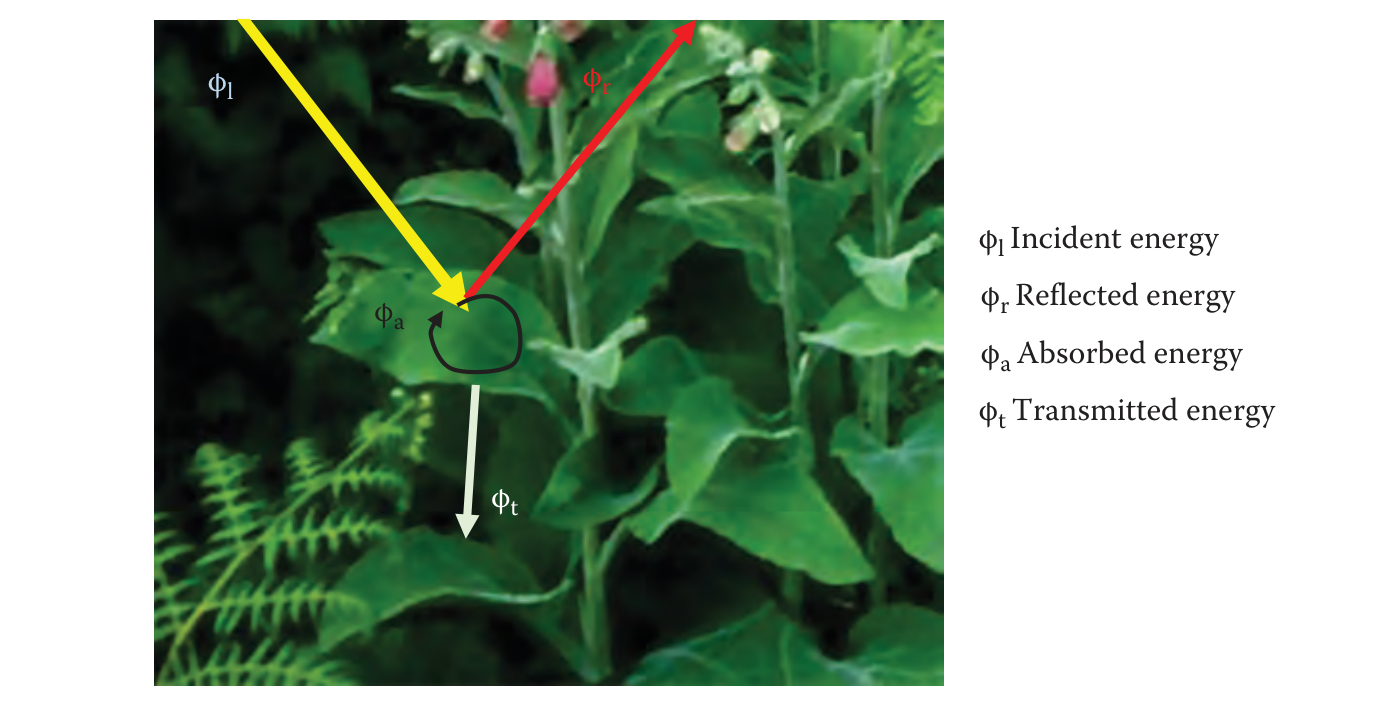
\includegraphics[width=0.95\textwidth]{Images/InteraccionSuperficie.png}
    \end{center}
    \caption{Interacción de la radiación electromagnética con la superficie terrestre.}
    \reference{Datos tomados de \citeA{chuvieco2016fundamentals}.}
    \label{fig:InteraccionSuperficie}
\end{figure}

La absorción ocurre cuando la radiación es asimilada por el objeto, la transmisión tiene lugar cuando la radiación atraviesa el objeto, y la reflexión sucede cuando la radiación rebota en el objetivo y es redirigida (ver Figura~\ref{fig:InteraccionSuperficie}). En el campo de la teledetección, se utiliza principalmente la radiación reflejada, ya que esta provee características significativas de la superficie terrestre al sensor remoto \cite{canada2007fundamentals, tempfli2009principles, chuvieco2016fundamentals}.

Existen dos tipos de reflexión: la reflexión especular y la reflexión difusa.

\textit{Reflexión especular}: Ocurre principalmente en superficies lisas, donde la radiación se refleja de manera casi uniforme en una sola dirección. Ejemplos comunes de esto incluyen la superficie del agua o el techo de un invernadero.

\textit{Reflexión difusa}: Tiene lugar cuando la superficie es rugosa, provocando que la radiación se refleje en múltiples direcciones de manera casi uniforme.

La manera en que un objeto refleja la radiación, ya sea de forma especular, difusa o una combinación de ambas, depende de la rugosidad de su superficie en relación con la longitud de onda de la radiación incidente \cite{tempfli2009principles}. La mayoría de las superficies exhiben características que se ubican en un punto intermedio entre estos dos extremos \cite{canada2007fundamentals}. Esta interacción singular da lugar a patrones de reflectancia que se identifican como ``firma espectral'', funcionando como una huella dactilar única para cada superficie y permitiendo su diferenciación e identificación \cite{chuvieco2016fundamentals}.

\subsubsection{Firma espectral}

La firma espectral, también denominada curva espectral, representa la cantidad de radiación incidente que se refleja en función de la longitud de onda, permitiendo así la identificación de objetos o materiales en una imagen de teledetección. Cada material posee una firma espectral única, determinada por sus propiedades físicas y químicas \cite{tempfli2009principles}. Por ejemplo, en el espectro visible y cercano al infrarrojo, la vegetación saludable suele reflejar gran cantidad de luz en las longitudes de onda verdes y del infrarrojo cercano, pero absorbe gran parte de la luz en las longitudes de onda rojas y azules. Esta interacción con la luz da a la vegetación su característico color verde \cite{emery2017introduction}.

Cada material posee una firma espectral única, determinada por sus características físicas y químicas \cite{chuvieco2016fundamentals}. Estas firmas permiten diferenciar diversos materiales presentes en una imagen de teledetección, facilitando así la elaboración de mapas que representan la distribución de estos materiales sobre la superficie terrestre (ver Figura \ref{fig:FirmasEspectralesSuperficie}).

\begin{figure}[H]
    \begin{center}
        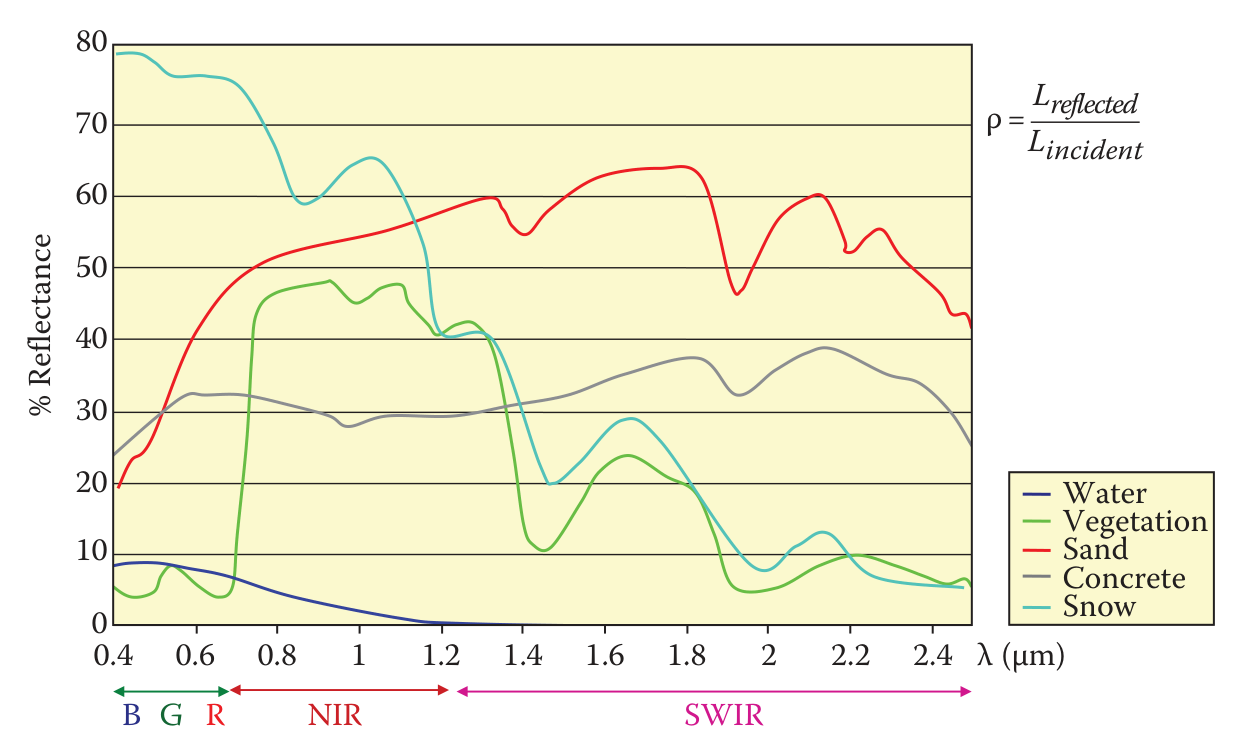
\includegraphics[width=1\textwidth]{Images/FirmasEspectralesSuperficie.png}
    \end{center}
    \caption{Firmas espectrales de los principales elementos de la superficie terrestre.}
    \reference{Datos tomados de \citeA{chuvieco2016fundamentals}.}
    \label{fig:FirmasEspectralesSuperficie}
\end{figure}

A pesar de que las firmas espectrales pueden facilitar la distinción entre diferentes materiales en la superficie terrestre, a menudo se encuentran diversos factores que pueden afectar su interpretación.

Tal como expone \citeA{chuvieco2016fundamentals}, existen múltiples elementos clave que pueden influir en las firmas espectrales (ver Figura~\ref{fig:FactorInfluenciaFirmasEspectrales}): (\textit{i}) Los componentes atmosféricos, que impactan en la absorción y dispersión de la radiación tanto entrante como reflejada. (\textit{ii}) Las variaciones en la cobertura del suelo que provocan cambios en la composición química o física, como por ejemplo la densidad, el contenido de pigmentos, la humedad o la rugosidad. Estas modificaciones pueden ser el resultado del ciclo estacional de la vegetación o los cultivos, las prácticas agrícolas, el pastoreo, entre otros. (\textit{iii}) El suelo y el sustrato geológico, especialmente importantes en áreas con cobertura vegetal limitada y dispersa, pues el sensor percibirá una señal más intensa procedente del suelo. (\textit{iv}) Las condiciones de iluminación solar, influenciadas por la latitud, el día del año y la hora del día. (\textit{v}) La pendiente del terreno. (\textit{vi}) El aspecto, que altera las condiciones de iluminación de una cobertura objetivo.

\begin{figure}[H]
    \begin{center}
        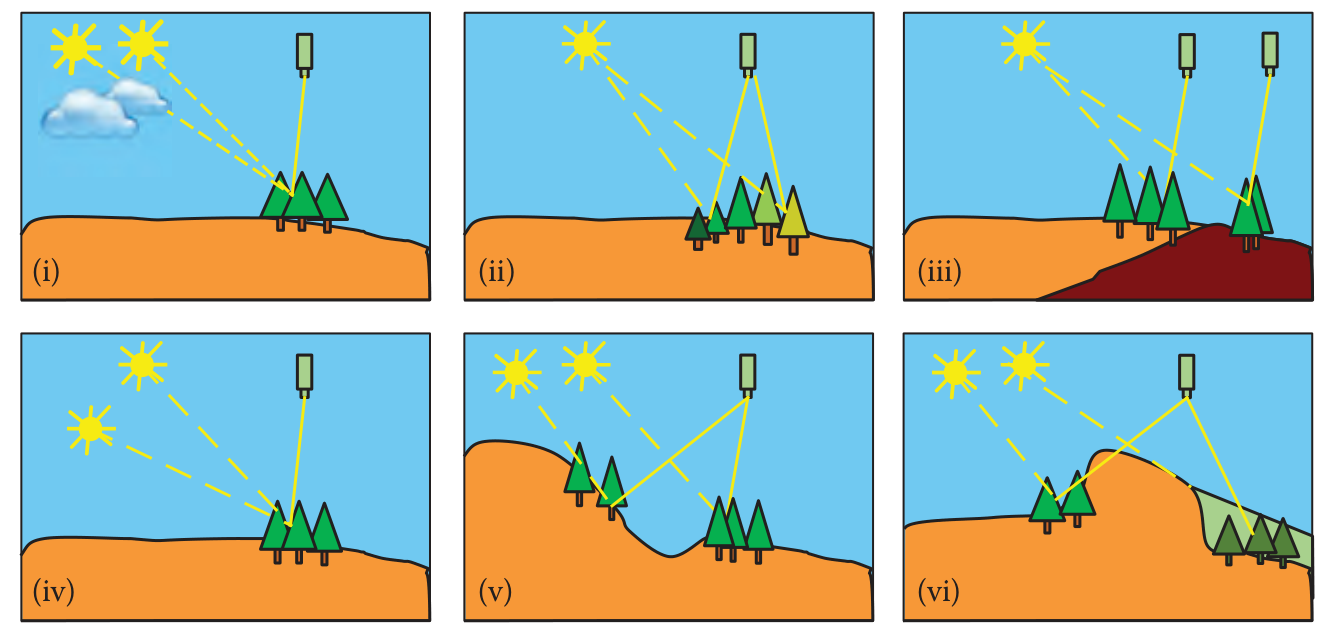
\includegraphics[width=1\textwidth]{Images/FactorInfluenciaFirmasEspectrales.png}
    \end{center}
    \caption{Factores que influencian en la composición de las firmas espectrales.}
    \reference{Datos tomados de \citeA{chuvieco2016fundamentals}.}
    \label{fig:FactorInfluenciaFirmasEspectrales}
\end{figure}

\subsubsection{Firmas espectrales}

\textbf{a) Vegetación}

La coloración verde característica de las plantas se debe en gran parte a la presencia de clorofila, un pigmento que absorbe entre un 60\% y 75\% de la energía en las longitudes de onda azul y roja \cite{chuvieco2016fundamentals}. La cantidad de clorofila varía a lo largo del año, siendo mayor o menor en las hojas según la estación. Además, las hojas sanas actúan como reflectores difusos en longitudes de onda cercanas al infrarrojo (NIR), aunque este comportamiento varía dependiendo del desarrollo de la hoja y su estructura celular. Este fenómeno permite medir y monitorear la salud de la vegetación \cite{canada2007fundamentals}. Adicionalmente, el contraste entre NIR y SWIR se utiliza a menudo para estimar el contenido de humedad de las hojas, ya que en el rango del SWIR, la reflectancia está mayormente determinada por la presencia de agua libre en el tejido de la hoja, de manera que una mayor cantidad de agua libre conlleva una menor reflectancia \cite{tempfli2009principles}.

\textbf{b) Agua}

Las longitudes de onda más largas del espectro visible y del infrarrojo cercano son absorbidas cuando interactúan con el agua, mientras que las longitudes de onda más cortas no, por lo que el agua se percibe de un tono azul o azul verdoso. El tinte verdoso es resultado de la presencia de algas en el agua, cuya clorofila absorbe más longitudes de onda azules y refleja las verdes \cite{canada2007fundamentals, tempfli2009principles}.

Comparada con la vegetación y los suelos, el agua tiene una reflectancia generalmente más baja. La vegetación puede reflejar hasta un 50\% de la energía incidente y los suelos hasta un 30-40\%, mientras que el agua apenas refleja un máximo del 10\%. La radiación reflejada por el agua se encuentra principalmente en el rango visible y, en menor grado, en el infrarrojo cercano, por lo que el resto de la energía es absorbida \cite{tempfli2009principles}.

Factores como la topografía y la presencia de sedimentos en la superficie del agua pueden dificultar la interpretación de las imágenes de teledetección debido a la reflexión especular, la cual afecta tanto el color como el brillo de la imagen \cite{canada2007fundamentals}. La rugosidad de la superficie del agua puede dar lugar a una reflexión difusa y dispersión, resultando en una mayor reflectancia. En aguas tranquilas, la reflexión es predominantemente especular, con una reflectancia altamente direccional y con valores variables dependiendo de los ángulos de visión y la dirección del sensor \cite{chuvieco2016fundamentals}.

\textbf{c) Hielo y nieve}

A diferencia del agua, la nieve exhibe una reflectancia muy elevada en las bandas visibles, disminuyendo considerablemente en el NIR y aún más en el SWIR. La reflectancia de la nieve está influenciada por factores como el tamaño de los cristales de nieve, la profundidad y densidad de la capa de nieve, así como la cantidad de impurezas que pueda contener. Cuando la nieve es más reciente, su reflectancia será mayor; por el contrario, será más baja a medida que envejece o se ensucia (ver Figura~\ref{fig:CurvasReflectanciaNieve}).

\begin{figure}[H]
    \begin{center}
        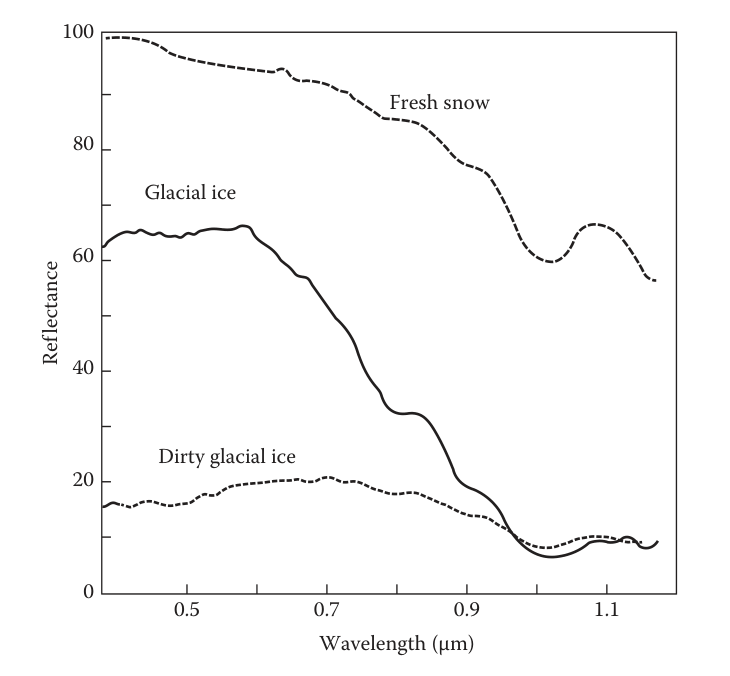
\includegraphics[width=0.8\textwidth]{Images/CurvasReflectancia.png}
    \end{center}
    \caption{Firma espectral de diferentes tipos de hielo y nieve.}
    \reference{Datos tomados de \citeA{chuvieco2016fundamentals}.}
    \label{fig:CurvasReflectanciaNieve}
\end{figure}

En el espectro visible, la nieve y las nubes suelen presentar retos para su diferenciación, debido a su similar alto índice de reflectancia. Sin embargo, este problema no persiste en el espectro SWIR. Los cristales de hielo o gotas de agua que constituyen las nubes son considerablemente más pequeños que los granos de nieve, resultando en una absorción menor de radiación en esta sección del espectro. A pesar de las dificultades en su identificación, la nieve por lo general exhibe una reflectancia ligeramente superior en las bandas visibles y una textura más uniforme en comparación a las nubes \cite{chuvieco2016fundamentals}.

\subsubsection{Características de la radiación electromagnética en la región del infrarrojo térmico del espectro electromagnético}

En la región del infrarrojo térmico (TIR) del espectro electromagnético, la radiación detectada por los sensores remotos proviene principalmente de la Tierra, ya que la reflexión de la radiación solar es mínima. Esto convierte la región del TIR en una herramienta útil para detectar cambios de temperatura en el suelo y la atmósfera.

La temperatura de un objeto está relacionada con su capacidad para absorber la radiación solar incidente. Si se considera que la suma de la reflectancia, transmisión y absorción es igual a 1, es decir, $1=\rho+\alpha+\tau$, y asumimos que la transmisión es $0$ en la región del TIR, la ecuación se simplifica a $1=\rho+\alpha$. Según la ley de Kirchhoff, la emisividad de un objeto es igual a su capacidad de absorción, lo que significa que cuanto mayor sea su absorción, mayor será su emisión. Por lo tanto, se llega a la siguiente ecuación:

\begin{equation}
    1=\rho+\epsilon
\end{equation}

donde:
\begin{itemize}
    \item $\rho$ es la reflectancia.
    \item $\epsilon$ es la emisividad del objeto.
\end{itemize}

Esto implica que los objetos con alta reflectancia absorberán poca radiación electromagnética y, como consecuencia, su nivel de emisividad será bajo. En la superficie terrestre, los elementos que emiten más son el agua y la vegetación densa, mientras que los suelos arenosos, la nieve y los metales muestran una emisividad menor.

Otros factores que influyen en el comportamiento térmico de un objeto son la capacidad térmica ($C$), la conductividad térmica ($k$), la difusividad térmica ($K$) y la inercia térmica ($P$) \cite{chuvieco2016fundamentals}.

En el Cuadro~\ref{tab:PropiedadesTIR} se detallan las propiedades de algunas de las coberturas de la superficie terrestre más comunes.

\begin{table}[H]
    \caption{Propiedades de las principales superficies terrestres en la región del infrarrojo térmico del espectro electromagnético.}
    \small
    \begin{tabularx}{1\textwidth}{lX}
        \hline
        \textbf{Superficie terrestre} & \textbf{Propiedades}                                                                                                                                                                                                                                                                                                                                                                                                                                                                                                                                                                        \\ \hline
        \textbf{Vegetación}           & La vegetación interactúa con una variedad de factores como la radiación solar, la fotosíntesis y la liberación de calor. Gracias a su alto contenido de agua, la vegetación presenta una considerable resistencia a los cambios bruscos de temperatura. Durante el día, la temperatura de las plantas tiende a disminuir debido a los procesos de transpiración. Por el contrario, durante la noche, la radiación absorbida durante el día se emite en forma de radiación térmica, lo que provoca un aumento en la temperatura de la vegetación, manteniendo así, su equilibrio energético. \\  \hline
        \textbf{Agua}                 & El agua presenta una notable resistencia a los cambios de temperatura debido a su alta conductividad térmica. La radiación incidente es absorbida de manera intensa y transmitida a lo largo de toda la superficie acuática. Este proceso contribuye a la notable estabilidad de la temperatura del agua.                                                                                                                                                                                                                                                                                   \\  \hline
        \textbf{Hielo y nieve}        & Las coberturas de nieve, debido a su menor emisividad de radiación electromagnética, registran temperaturas más bajas en comparación con su entorno. Esto se debe no solo a su alta reflectancia, sino también a otros factores como el tamaño de los cristales de nieve y su contenido de agua.                                                                                                                                                                                                                                                                                            \\  \hline
    \end{tabularx}
    \begin{minipage}{\textwidth}
        \vspace{10pt}
        \reference{Datos tomados de \cite{chuvieco2016fundamentals}.}
        \label{tab:PropiedadesTIR}
    \end{minipage}
\end{table}

\subsubsection{Características de la radiación electromagnética en la región de las microondas del espectro electromagnético}

Las microondas representan la región del espectro electromagnético que contiene longitudes de onda más largas. Esta región se diferencia de las mencionadas anteriormente, debido a que no depende de datos ópticos, es decir, datos derivados de la luz visible o cercana a esta \cite{tempfli2009principles}.

En la teledetección, las microondas se segmentan en diversas sub regiones según su longitud de onda. Cada una de estas sub regiones se representan mediante un carácter alfabético, como se muestra en el Cuadro~\ref{tab:BandasMW}.

\begin{table}[H]
    \caption{Representación de las sub regiones de las microondas utilizadas en la teledetección.}
    \small
    \begin{tabularx}{1\textwidth}{Xccc}
        \hline
        \textbf{Nombre \hspace{1cm}} & \textbf{\hspace{0.5cm}Longitud ($cm$)\hspace{0.5cm}} & \textbf{\hspace{0.5cm}Valor central ($cm$)\hspace{0.5cm}} & \textbf{Frecuencia ($GHz$)} \\ \hline
        $Ka$                         & 0.75 - 1.10                                          &                                                           &                             \\
        $K$                          & 1.10 - 1.67                                          & 1.0                                                       & 10.9 - 36                   \\
        $Ku$                         & 1.67 - 2.40                                          &                                                           &                             \\ \hline
        $X$                          & 2.40 - 3.75                                          & 3.0                                                       & 5.75 - 10.90                \\ \hline
        $C$                          & 3.75 - 7.50                                          & 5.6                                                       & 3.90 - 5.75                 \\ \hline
        $S$                          & 7.50 - 15.00                                         & 10.0                                                      & 1.55 - 3.90                 \\ \hline
        $L$                          & 15.00 - 30.00                                        & 23.0                                                      & 0.39 - 1.55                 \\ \hline
        $P$                          & 30.00 - 100.00                                       & 70.0                                                      & > 0.39                      \\ \hline
    \end{tabularx}
    \begin{minipage}{\textwidth}
        \vspace{10pt}
        \reference{Datos tomados de \cite{chuvieco2016fundamentals}.}
        \label{tab:BandasMW}
    \end{minipage}
\end{table}

Una de las principales características de esta región es su alta capacidad de transmisión atmosférica, lo que significa que es posible observar áreas sin importar las condiciones climáticas, superando así limitaciones comunes de otros métodos de teledetección, esto es debido a que las longitudes de onda son más grandes que el tamaño promedio de las partículas y moléculas presentes en la atmósfera (ver Figura~\ref{fig:LongitudOndaMW}).

\begin{figure}[H]
    \begin{center}
        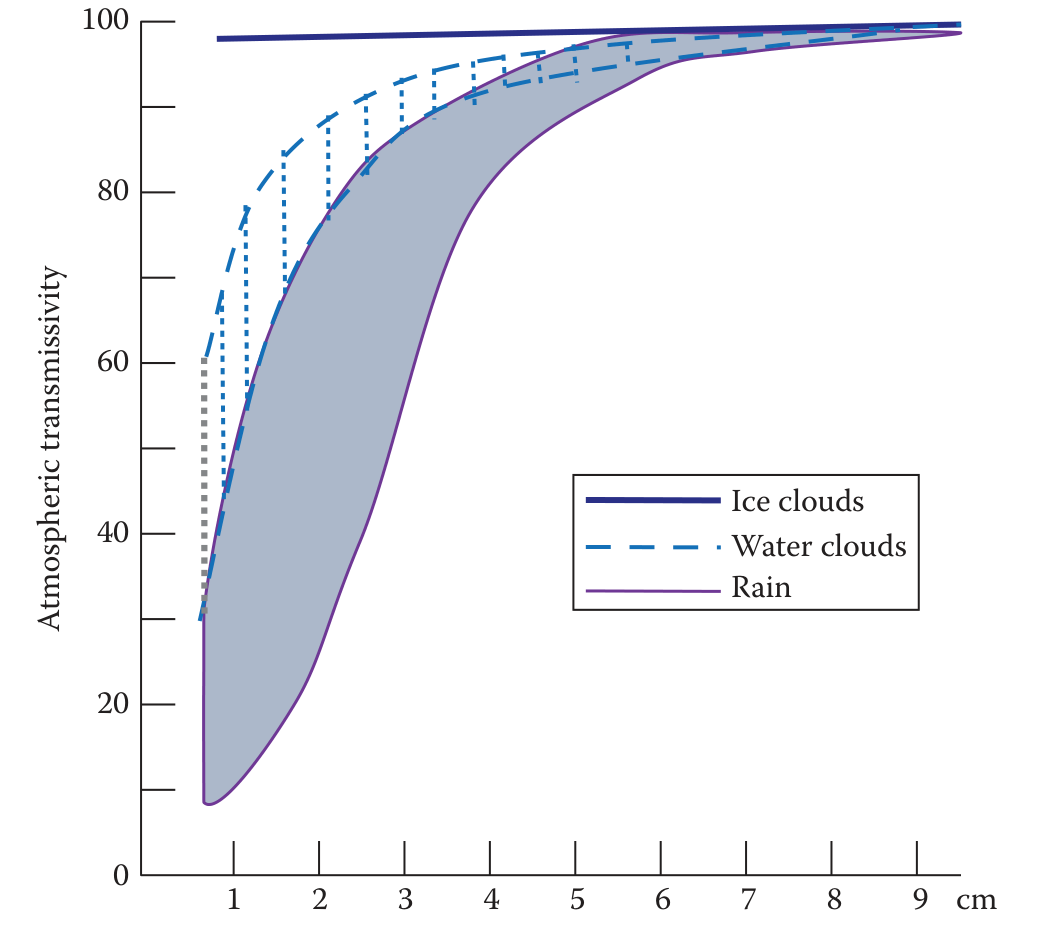
\includegraphics[width=0.8\textwidth]{Images/LongitudOndaMW.png}
    \end{center}
    \caption{Capacidad de transmisión atmosférica en la región de las microondas.}
    \reference{Datos tomados de \citeA{chuvieco2016fundamentals}.}
    \label{fig:LongitudOndaMW}
\end{figure}

Las observaciones remotas en esta región espectral se realizan mayormente con sensores activos, como el radar, que emiten y detectan energía de microondas desde la superficie. No obstante, también existen radiómetros pasivos de microondas, que recogen radiación de la superficie de forma similar a los sensores ópticos \cite{chuvieco2016fundamentals}.

En el Cuadro~\ref{tab:PropiedadesMW} se detallan las propiedades de algunas de las coberturas de la superficie terrestre más comunes.

\begin{table}[H]
    \caption{Propiedades de las principales superficies terrestres en la región de las microondas del espectro electromagnético.}
    \small
    \begin{tabularx}{1\textwidth}{lX}
        \hline
        \textbf{Superficie terrestre} & \textbf{Propiedades}                                                                                                                                                                                                                                                                                                                                                                                                                                                                                                                                                                                                                                                    \\ \hline
        \textbf{Vegetación}:          & La vegetación tiende a tener una respuesta espectral en la región de las microondas que es bastante compleja y depende de varios factores, incluyendo el tipo de vegetación, su etapa de crecimiento, y las condiciones ambientales. La vegetación, debido a su estructura tridimensional (hojas, ramas y tallos), interactúa con las microondas de una manera característica que se puede detectar. Las ondas de microondas pueden penetrar la vegetación y reflejar de manera más fuerte las estructuras más densas, como el tallo y las ramas de los árboles. Esta capacidad de penetración también permite la detección de la humedad del suelo bajo la vegetación.
        \\  \hline
        \textbf{Agua}:                & El agua, especialmente el agua de mar, tiene una firma espectral muy baja en la región de las microondas debido a su alta capacidad para absorber las ondas de radio. Por eso, los cuerpos de agua suelen aparecer muy oscuros en las imágenes de radar. La superficie del agua puede reflejar las microondas, pero la señal que llega al sensor es muy débil debido a la absorción.                                                                                                                                                                                                                                                                                    \\  \hline
        \textbf{Hielo y nieve}:       & Los sensores de microondas pasivos son muy útiles para monitorear el hielo marino, ya que son más sensibles a las temperaturas frías que los sensores ópticos. El hielo marino y el hielo de agua dulce también tienen firmas espectrales distintas debido a las diferencias en su estructura y composición.                                                                                                                                                                                                                                                                                                                                                            \\  \hline
    \end{tabularx}
    \begin{minipage}{\textwidth}
        \vspace{10pt}
        \reference{Datos tomados de \cite{chuvieco2016fundamentals}.}
        \label{tab:PropiedadesMW}
    \end{minipage}
\end{table}

\subsubsection{Plataformas}

Las plataformas son consideradas vehículos en movimiento, tales como satélites, aviones o vehículos aéreos no tripulados, empleados para diversas actividades específicas y conformados por diversos equipos o instrumentos \cite{tempfli2009principles}. Son de vital importancia ya que alojan los sensores encargados de obtener la información de la radiación electromagnética reflejada o incidente desde la Tierra \cite{chuvieco2016fundamentals}.

En función de su localización, las plataformas de teledetección se clasifican en terrestres, aéreas y espaciales \cite{canada2007fundamentals}. La utilidad de cada tipo de plataforma se determina según las necesidades específicas de la aplicación en cuestión. En el contexto de la teledetección, estas plataformas pueden operar desde alturas tan bajas como unos pocos centímetros, con el uso de equipamiento de campo, hasta posiciones en órbitas geoestacionarias a aproximadamente 36,000 km de distancia de la Tierra (ver Figura~\ref{fig:PlataformasTeledeteccion}) \cite{tempfli2009principles}.

\begin{figure}[H]
    \begin{center}
        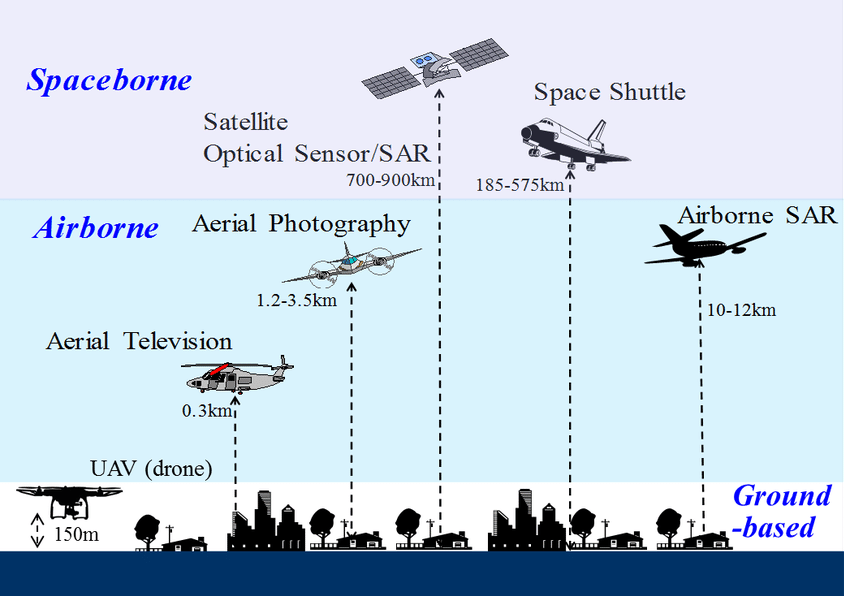
\includegraphics[width=1\textwidth]{Images/Plataformas.png}
    \end{center}
    \caption{Plataformas de teledetección.}
    \reference{Datos tomados de \citeA{yamazaki2016remote}.}
    \label{fig:PlataformasTeledeteccion}
\end{figure}

\textbf{a) Plataformas terrestres:} Conocidas también como \textit{Ground-based} en la jerga anglosajona, las plataformas terrestres ofrecen un alto nivel de detalle sobre zonas específicas, gracias a la cercanía entre el sensor y el área objeto de estudio. Comúnmente, se emplean estructuras elevadas como torres, edificios o grúas para su instalación \cite{canada2007fundamentals}. No obstante, esta categoría también abarca vehículos aéreos no tripulados, conocidos como Drones, que operan a una altitud máxima de aproximadamente 150 metros desde el nivel del suelo \cite{yamazaki2016remote}.

\textbf{b) Plataformas aéreas:} En inglés se denominan \textit{Airborne}. Aeronaves, sean aviones de ala fija o helicópteros, ofrecen la capacidad de cubrir vastas áreas geográficas en un tiempo relativamente corto. Operan a altitudes que van desde los 0.3 km hasta los 12 km sobre la superficie terrestre \cite{tempfli2009principles, yamazaki2016remote}. La flexibilidad en velocidad y altitud de estos vehículos influye directamente en la resolución y la escala de las imágenes obtenidas \cite{canada2007fundamentals}. Sin embargo, elementos como el viento y la orientación del vehículo pueden afectar la calidad del dato recogido \cite{tempfli2009principles}.

\textbf{c) Plataformas espaciales:} O \textit{Spaceborne} en inglés, proporcionan una perspectiva más global y tienen la ventaja de capturar datos de manera continua debido a sus órbitas específicas. Los satélites son los más comunes en esta categoría y suelen orbitar entre 700 y 900 km de altura respecto a la superficie terrestre. También existen vehículos espaciales que operan a altitudes que van desde los 185 hasta los 575 km desde la superficie terrestre \cite{tempfli2009principles}.

Los sensores terrestres son usualmente más asequibles pero tienen una cobertura limitada. Las plataformas aéreas ofrecen más flexibilidad pero incurren en mayores costos. Los satélites, aunque representan una inversión significativa, brindan la ventaja de un alcance global y una recopilación de datos constante \cite{canada2007fundamentals}.

\subsubsection{Sensores}

Los sensores en teledetección son dispositivos ubicados en plataformas de observación que miden y almacenan información a partir de la radiación electromagnética reflejada o emitida por la Tierra \cite{tempfli2009principles}.

\begin{figure}[H]
    \begin{center}
        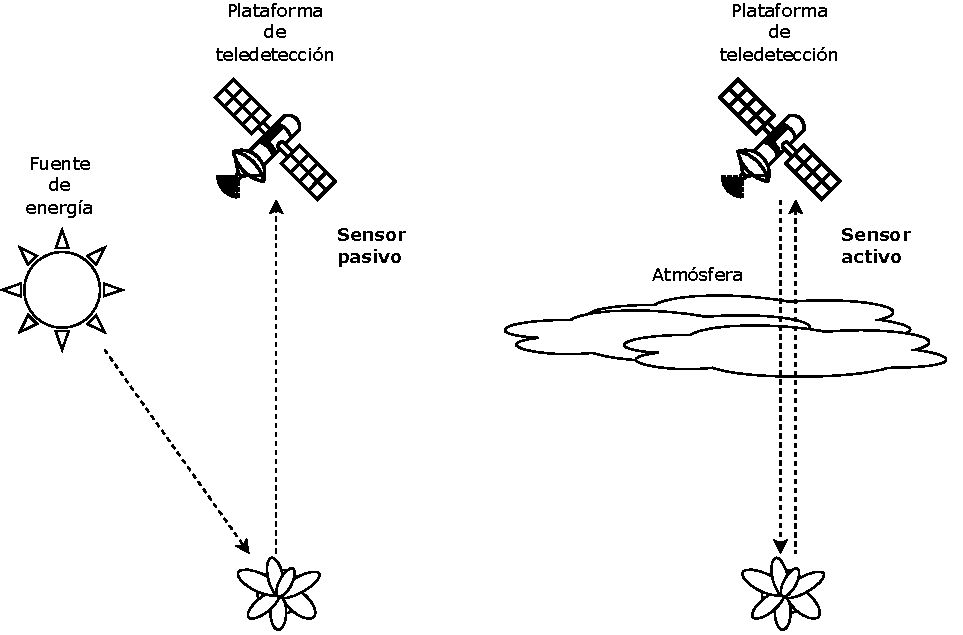
\includegraphics[width=1\textwidth]{Images/TipoSensores.pdf}
    \end{center}
    \caption{Tipos de sensores.}
    \reference{Elaborado por el autor.}
    \label{fig:TipoSensores}
\end{figure}

\textbf{a) Tipos de sensores}

Un enfoque habitual para clasificar los sensores en teledetección es según el método que emplean para captar información de la radiación electromagnética. Bajo este criterio, se distinguen principalmente dos tipos de sensores: activos y pasivos \cite{chuvieco2016fundamentals}.

\begin{itemize}
    \item \textit{Sensores pasivos:} Como se mencionó anteriormente, el Sol es la principal fuente de radiación electromagnética en la teledetección, lo que lo convierte en una fuente natural de energía. Estos sensores dependen de fuentes externas de energía como el Sol y, en algunos casos, la energía térmica de la Tierra (ver Figura~\ref{fig:TipoSensores}).

          Cubren un rango en el espectro electromagnético que va desde los rayos gamma hasta las microondas. Los ejemplos más comunes y antiguos de este tipo de sensores son las cámaras fotográficas y los escáneres electro ópticos \cite{tempfli2009principles, chuvieco2016fundamentals}. Sin embargo, tienen limitaciones; por ejemplo, su disponibilidad es limitada durante la noche, y su calidad depende de las condiciones climáticas de la atmósfera terrestre. Además, la radiación térmica emitida por la Tierra debe ser lo suficientemente intensa como para ser detectada por el sensor \cite{canada2007fundamentals}.

    \item \textit{Sensores activos:} La principal característica de este tipo de sensores es que son su propia fuente de energía (ver Figura~\ref{fig:TipoSensores}). Por lo tanto, las mediciones no dependen de factores externos como la luminosidad y el clima. Entre ellos se incluyen imágenes de Radar, LiDAR y Sonar. Un uso común de estos productos es para imágenes que representan altimetría \cite{tempfli2009principles, chuvieco2016fundamentals}.

          Estos sensores permiten obtener información de la radiación reflejada en cualquier momento del día y en cualquier estación del año. Además, tienen la capacidad de emitir radiación electromagnética en diversas longitudes de onda, a diferencia del Sol. Por ejemplo, las microondas pueden atravesar fácilmente la atmósfera terrestre gracias a su longitud de onda \cite{canada2007fundamentals}.
\end{itemize}

\subsubsection{Imágenes de teledetección}

La radiación electromagnética puede ser registrada tanto en fotografías como en imágenes. Tal como indica \citeA{canada2007fundamentals}, las imágenes y las fotografías presentan diferencias significativas. Las imágenes son representaciones digitales capturadas por cualquier tipo de dispositivo y pueden abarcar cualquier longitud de onda. Por otro lado, las fotografías se encuentran típicamente dentro del espectro visible y el infrarrojo, usualmente en un rango que va de $0.3 \mu m$ a $0.9 \mu m$.


\begin{figure}[H]
    \begin{center}
        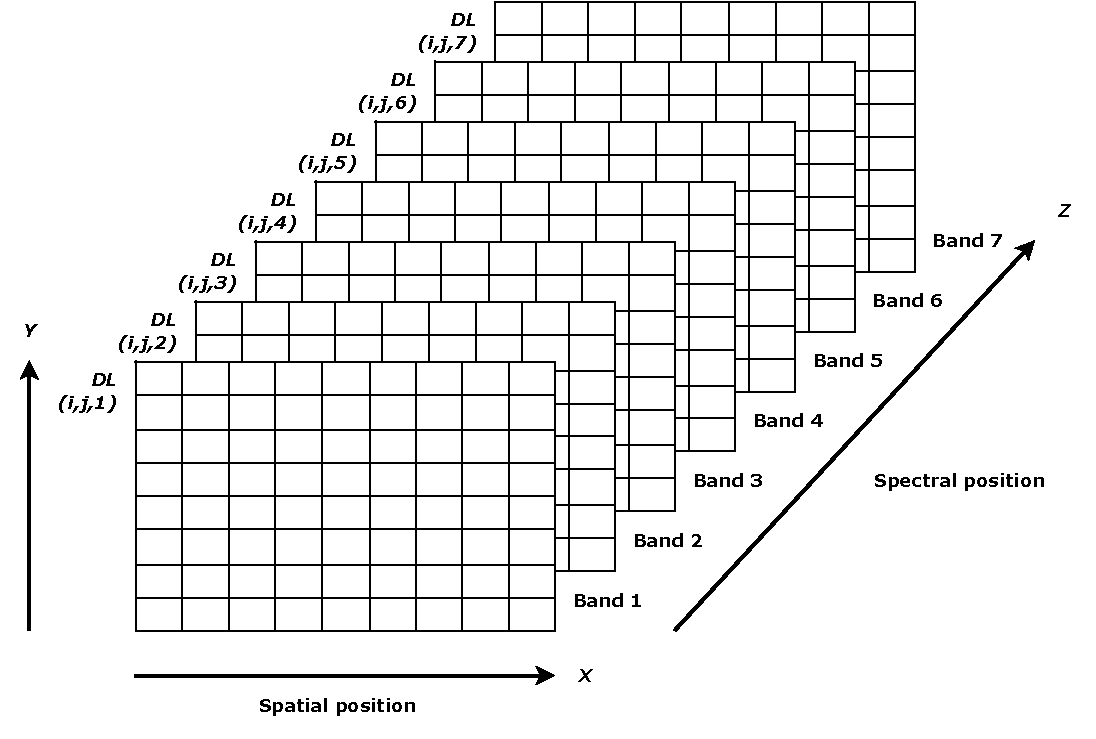
\includegraphics[width=1\textwidth]{Images/imagen_satelital.pdf}
    \end{center}
    \caption{Estructura y organización de los datos numéricos dentro de una imagen digital.}
    \reference{Datos tomados de \citeA{chuvieco2016fundamentals}.}
    \label{fig:ComposicionImagenSatelital}
\end{figure}

Las fotografías son consideradas imágenes, sin embargo, no todas las imágenes son necesariamente fotografías. En el ámbito digital, particularmente en teledetección, las imágenes se representan mediante matrices numéricas. Cada número de esta matriz corresponde a un píxel, la unidad más pequeña de una imagen. La Figura~\ref{fig:ComposicionImagenSatelital} ilustra cómo una imagen puede descomponerse en una matriz numérica en los ejes X e Y. Si la imagen tiene varias bandas, adquiere una estructura tridimensional en la que el eje Z representa diferentes bandas espectrales, lo cual es común en imágenes de teledetección ópticas \cite{chuvieco2016fundamentals}.

\textbf{a) Resolución de imágenes}

La teledetección se caracteriza por distintas modalidades de resolución que determinan su capacidad para captar y representar detalles en las imágenes. Uno de los aspectos más relevantes es la \emph{resolución espacial}.

\begin{itemize}
    \item \textit{Resolución espacial:} Se refiere al tamaño del píxel, expresado generalmente en metros, que indica la habilidad del sensor para discernir el objeto más pequeño en una imagen \cite{chuvieco2016fundamentals}. Esta resolución no sólo es una función del diseño del sensor, sino que está influenciada por la distancia entre el sensor y el objetivo. Específicamente, un sensor situado a una mayor altitud podrá abarcar un área geográfica más extensa en su toma, pero, con frecuencia, compromete la precisión en los detalles más finos. Por otro lado, aquellos sensores más cercanos al terreno, aunque limitados en la extensión del área que registran, son capaces de proporcionar un nivel de detalle notablemente superior \cite{canada2007fundamentals}.

          \begin{figure}[H]
              \begin{center}
                  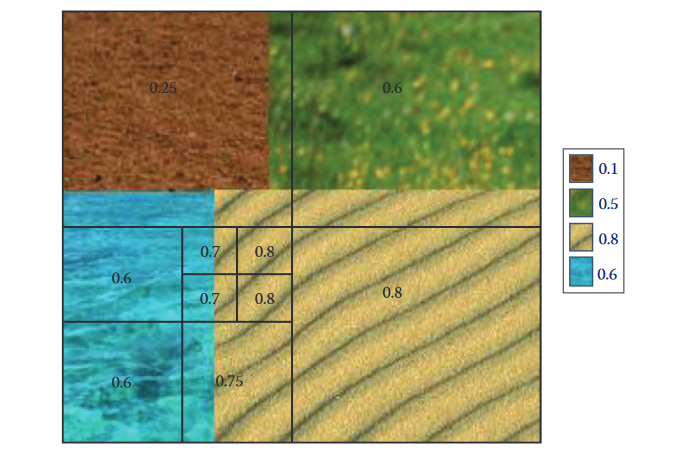
\includegraphics[width=1\textwidth]{Images/ResolucionEspacial.png}
              \end{center}
              \caption{Relación entre el tamaño del píxel y la capacidad de discriminación de los objetos en una imagen de teledetección.}
              \reference{Datos tomados de \citeA{chuvieco2016fundamentals}.}
              \label{fig:ResolucionEspacial}
          \end{figure}

          La elección adecuada de un sensor, en términos de su resolución espacial, es fundamental y debe estar alineada con los requerimientos específicos del estudio o aplicación en cuestión. Asimismo, es importante considerar que la resolución espacial incide directamente en la interpretación de las imágenes: mientras que imágenes de baja resolución son útiles para identificar características de mayor tamaño, aquellas con alta resolución permiten una detección e identificación más precisa de objetos más pequeños (ver Figura~\ref{fig:ResolucionEspacial}) \cite{canada2007fundamentals}.

    \item \textit{Resolución espectral:} Se refiere a la capacidad de un sensor para discernir la cantidad y el ancho de banda de los canales espectrales. Los sensores que cuentan con una elevada resolución espectral son capaces de identificar numerosas bandas delgadas a lo largo del espectro electromagnético. Sin embargo, aquellos sensores con resolución espectral más limitada perciben un número menor de bandas, que resultan ser más anchas \cite{chuvieco2016fundamentals}.

          \begin{figure}[H]
              \begin{center}
                  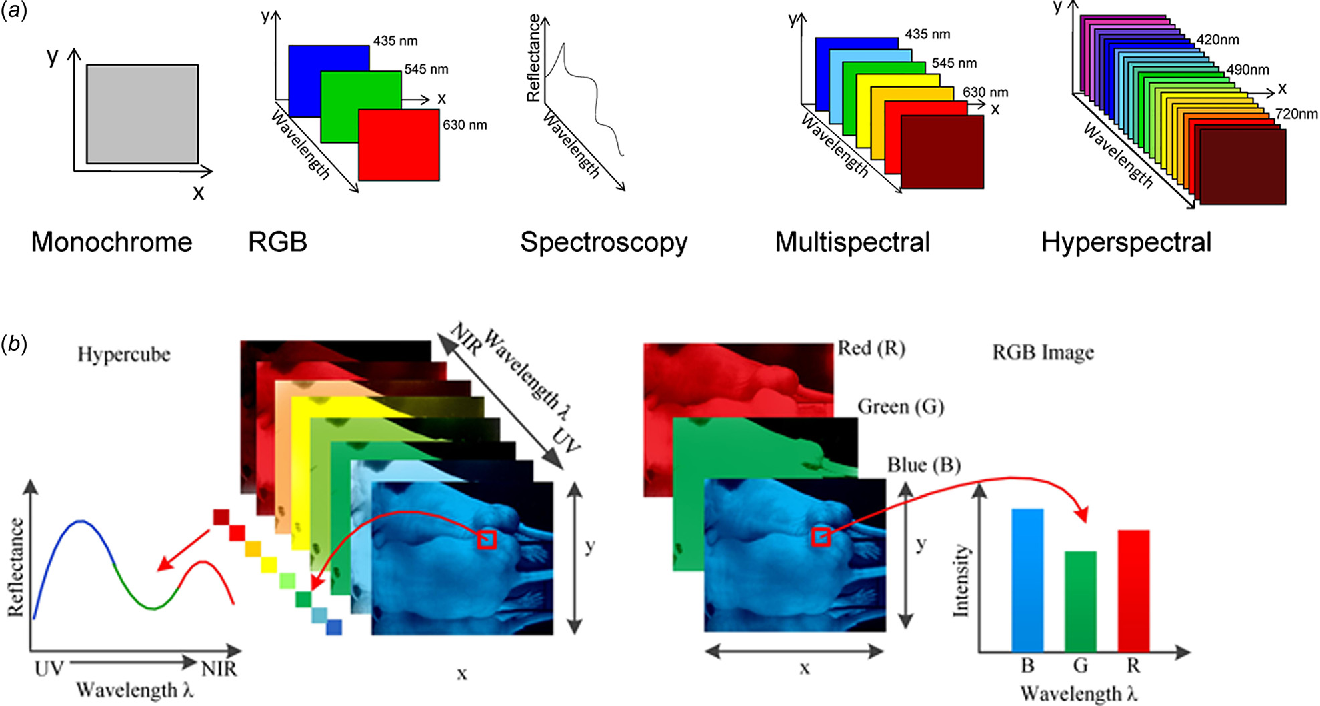
\includegraphics[width=1\textwidth]{Images/ResolucionEspectral.png}
              \end{center}
              \caption{Tipos de resolución espectral en una imagen de teledetección.}
              \reference{Datos tomados de \citeA{mehta2018single}.}
              \label{fig:ResolucionEspectral}
          \end{figure}

          En la actualidad se pueden encontrar imágenes con una sola banda espectral, imágenes con las bandas del espectro visible, y según aumente su cantidad de canales, imágenes multiespectrales e imágenes hiperespectrales (ver Figura~\ref{fig:ResolucionEspectral}).

    \item \textit{Resolución radiométrica:} La resolución radiométrica indica la capacidad de un sensor para distinguir minúsculas variaciones en la radiancia espectral. En sistemas fotográficos, determina la cantidad de niveles de grises que pueden ser almacenados. En sensores ópticos electrónicos, esta resolución establece el rango de valores usados para registrar la radiación electromagnética entrante \cite{chuvieco2016fundamentals}. Computacionalmente, un valor se representa como un «0» o un «1». Si se dice que una imagen es de 8 bits, esto supone un total de \(2^8\) o 256 posibles combinaciones (lo que indica el rango de valores que puede tomar el píxel) \cite{tempfli2009principles}.

          \begin{figure}[H]
              \begin{center}
                  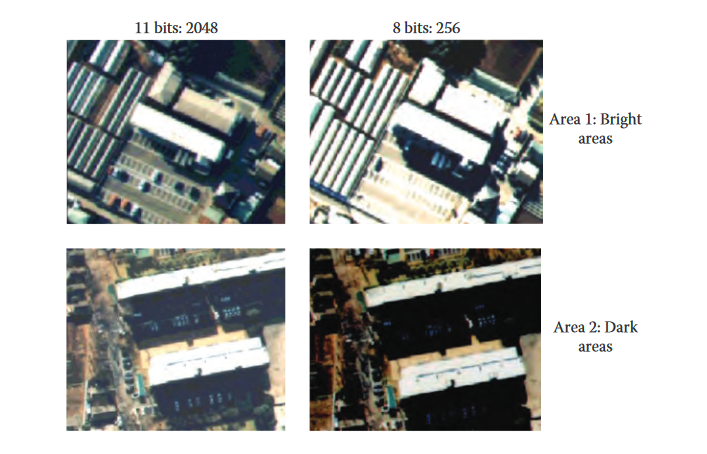
\includegraphics[width=1\textwidth]{Images/ResolucionRadiometrica.png}
              \end{center}
              \caption{Comparación visual de imágenes con diferentes resoluciones radiométricas (11 bits y 8 bits).}
              \reference{Datos tomados de \citeA{chuvieco2016fundamentals}.}
              \label{fig:ResolucionRadiometrica}
          \end{figure}

          Como señala \citeA{chuvieco2016fundamentals}, la resolución radiométrica es crucial en el análisis digital en comparación con el análisis visual. Esto se debe a que el ojo humano solo puede discernir alrededor de 64 niveles de gris y no más de 200.000 colores. Sin embargo, en sistemas de análisis digitales, esta resolución es fundamental para diferenciar objetos con firmas espectrales semejantes, tarea que sería inviable con sensores de menor sensibilidad tal y como se muestra en la Figura~\ref{fig:ResolucionRadiometrica}.

    \item \textit{Resolución temporal:} Hace referencia a la periodicidad con la que un satélite pasa por un punto específico de la superficie terrestre, es decir, el intervalo de tiempo entre dos observaciones consecutivas del mismo lugar \cite{tempfli2009principles, chuvieco2016fundamentals}. Esta resolución es importante para monitorear fenómenos en constante cambio, como el desarrollo de cultivos o la expansión urbana. Por ejemplo, el seguimiento de fenómenos climáticos rápidos requiere resoluciones temporales cortas, mientras que el estudio de cambios geológicos puede basarse en observaciones más espaciadas \cite{canada2007fundamentals}.
\end{itemize}

\textbf{b) Tipos de imágenes}

Las imágenes obtenidas a través de la teledetección se diferencian principalmente por los sensores que se utilizan en su captura. Los principales tipos se detallan en el Cuadro~\ref{tab:TiposImagenesTeledeteccion}.

\begin{table}[H]
    \caption{Tipos de imágenes de teledetección.}
    \begin{tabularx}{1\textwidth}{p{4.5cm}X}
        \hline
        \textbf{Tipo de imagen}                       & \textbf{Descripción}                                                                                                                                                                                                                                                                              \\
        \hline
        Imagen multiespectral                         & Imágenes de múltiples bandas donde cada píxel representa la información de la radiancia o reflectancia de los objetos en la superficie terrestre.                                                                                                                                                 \\
        \hline
        Imagen pancromática                           & Imágenes de una banda que integran la información de las bandas del espectro visible e infrarrojo cercano, comúnmente con una mayor resolución espacial que las imágenes multiespectrales.                                                                                                        \\
        \hline
        Imagen fusionada \newline (Pan-Sharpened)     & Resultado de la fusión entre una imagen pancromática y una multiespectral. Se mantiene la resolución espacial de la imagen pancromática, pero se incorporan los valores del sensor multiespectral en cada banda. Esta combinación se logra mediante un proceso denominado ``Pansharpening''.      \\
        \hline
        Imagen de radar                               & Las imágenes de radar de apertura sintética (SAR) provienen de sensores activos y se generan a partir de datos en el rango de las microondas. Estas ondas pueden penetrar la atmósfera y proporcionar información independientemente de condiciones climáticas, nubosidad o visibilidad nocturna. \\
        \hline
        Imágenes termográficas                        & Provienen de sensores térmicos que proporcionan información sobre la temperatura de la superficie terrestre.                                                                                                                                                                                      \\
        \hline
        Modelos digitales de elevación \newline (DEM) & Son representaciones digitales de la altitud superficial de una zona determinada. Se obtienen mediante el procesamiento de fotografías aéreas, imágenes SAR, imágenes LiDAR o datos topográficos. Entre los modelos digitales de elevación más empleados se encuentran: SRTM y ASTER GDEM.        \\
        \hline
    \end{tabularx}
    \begin{minipage}{\textwidth}
        \vspace{10pt}
        \reference{Datos tomados de \citeA{bravo2017teledeteccion}.}
        \label{tab:TiposImagenesTeledeteccion}
    \end{minipage}
\end{table}